\documentclass[aspectratio=169]{beamer}
%
% Choose how your presentation looks.
%
% For more themes, color themes and font themes, see:
% http://deic.uab.es/~iblanes/beamer_gallery/index_by_theme.html
%
\mode<presentation>
{
    \usetheme{default}      % or try Darmstadt, Madrid, Warsaw, ...
    \usecolortheme{default} % or try albatross, beaver, crane, ...
    \usefonttheme{default}  % or try serif, structurebold, ...
    \setbeamertemplate{navigation symbols}{}
    \setbeamertemplate{caption}[numbered]
}

\usepackage[english]{babel}
\usepackage[utf8]{inputenc}
\usepackage{graphicx}
\usepackage{breqn}
\usepackage{bbm}
%\usepackage{enumitem}

\newenvironment{wideitemize}{\itemize\addtolength{\itemsep}{10pt}}{\enditemize}

\DeclareMathOperator*{\argmax}{arg\,max}
\DeclareMathOperator*{\argmin}{arg\,min}

\usepackage[style=authoryear, backend=biber]{biblatex}
\addbibresource{}

\title{Selection Out of the US Federal Workforce}
\author{Nathaniel Bechhofer \and Churn Ken Lee}
\institute{UC San Diego}
\date{}

\begin{document}

\begin{frame}
    \titlepage
\end{frame}

\begin{frame}
    \frametitle{Data}

    \begin{wideitemize}
        \item Buzzfeed FOIA payroll data for federal government employees
        \item Employees from 1973 onwards
        \item Occupation, pay, tenure, (some) demographic information
        \item Flows since 1982
        \item Data since 2014 has employee ID withheld, so matching after 2014 using ID is not possible
    \end{wideitemize}

\end{frame}

\begin{frame}
    \frametitle{Question}

    Is there negative selection due to shutdowns and furloughs?

\end{frame}

\begin{frame}
    \frametitle{Why do we care?}

    \begin{wideitemize}
        \item 
    \end{wideitemize}

\end{frame}

\begin{frame}
    \frametitle{Separation rates over time}

    \begin{figure}[]
        \centering
        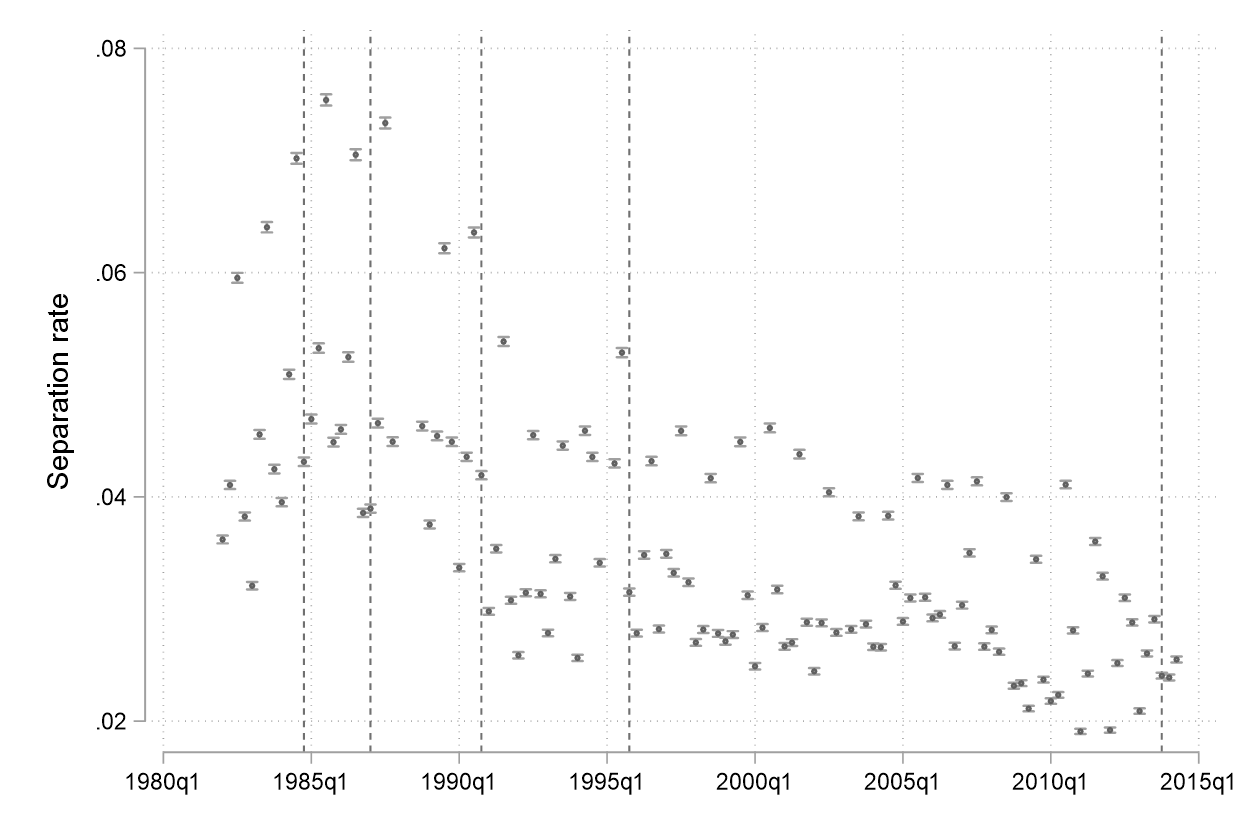
\includegraphics[width=0.8\textwidth]{../output/separation_rate_CI.png}
    \end{figure}

\end{frame}

\begin{frame}
    \frametitle{Separation rates over time, adjusted for linear time trend and seasonality}

    \begin{figure}[]
        \centering
        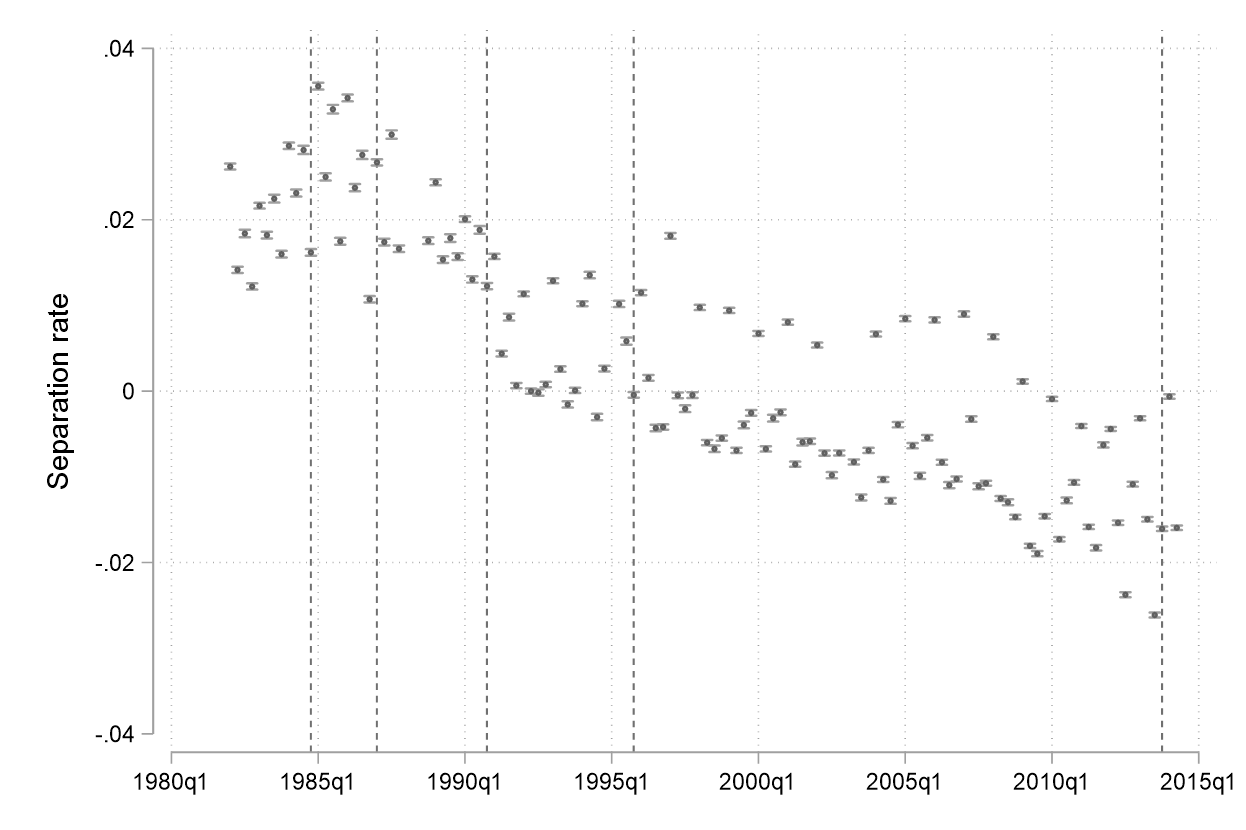
\includegraphics[width=0.8\textwidth]{../output/separation_rate_adj_CI.png}
    \end{figure}

\end{frame}

\begin{frame}
    \frametitle{Accession rates over time}

    \begin{figure}[]
        \centering
        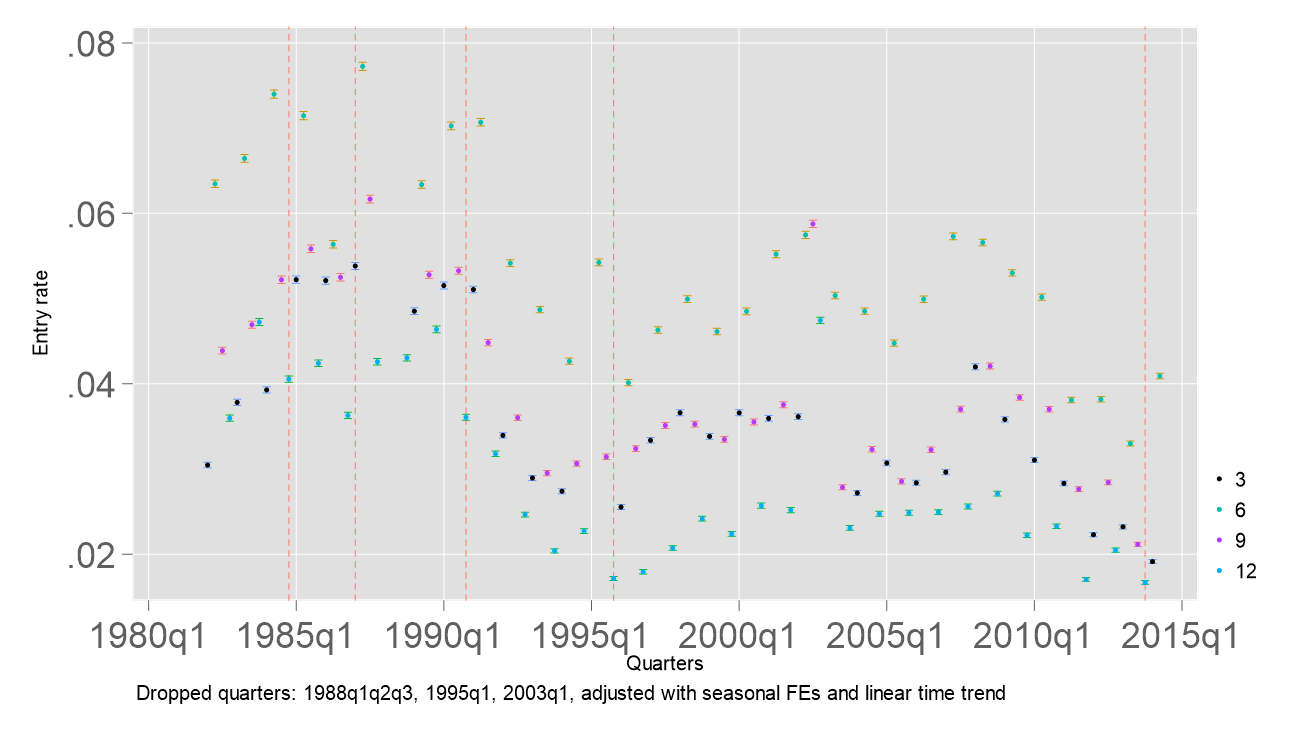
\includegraphics[width=0.8\textwidth]{../output/accession_rate_CI.png}
    \end{figure}

\end{frame}

\begin{frame}
    \frametitle{Accession rates over time, adjusted for linear time trend and seasonality}

    \begin{figure}[]
        \centering
        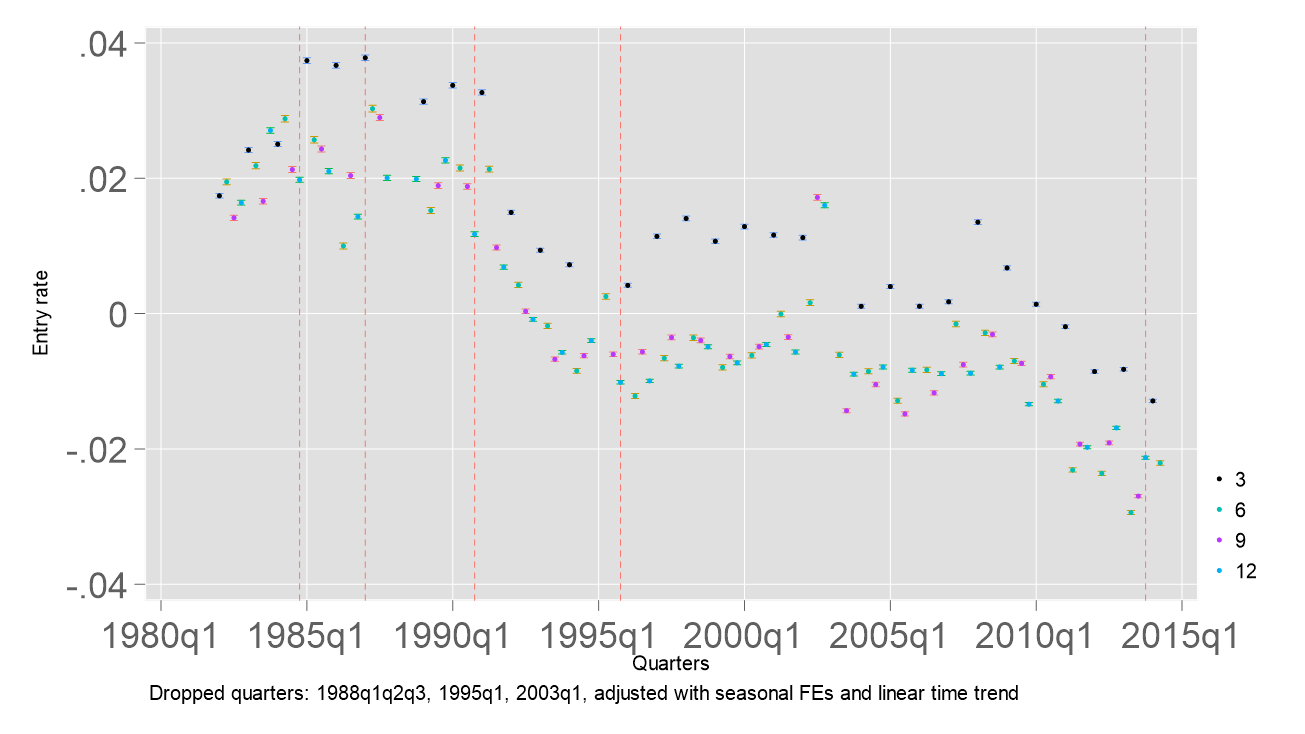
\includegraphics[width=0.8\textwidth]{../output/accession_rate_adj_CI.png}
    \end{figure}

\end{frame}

\begin{frame}
    \frametitle{Difference in separation rates over time by education}

    \begin{figure}[]
        \centering
        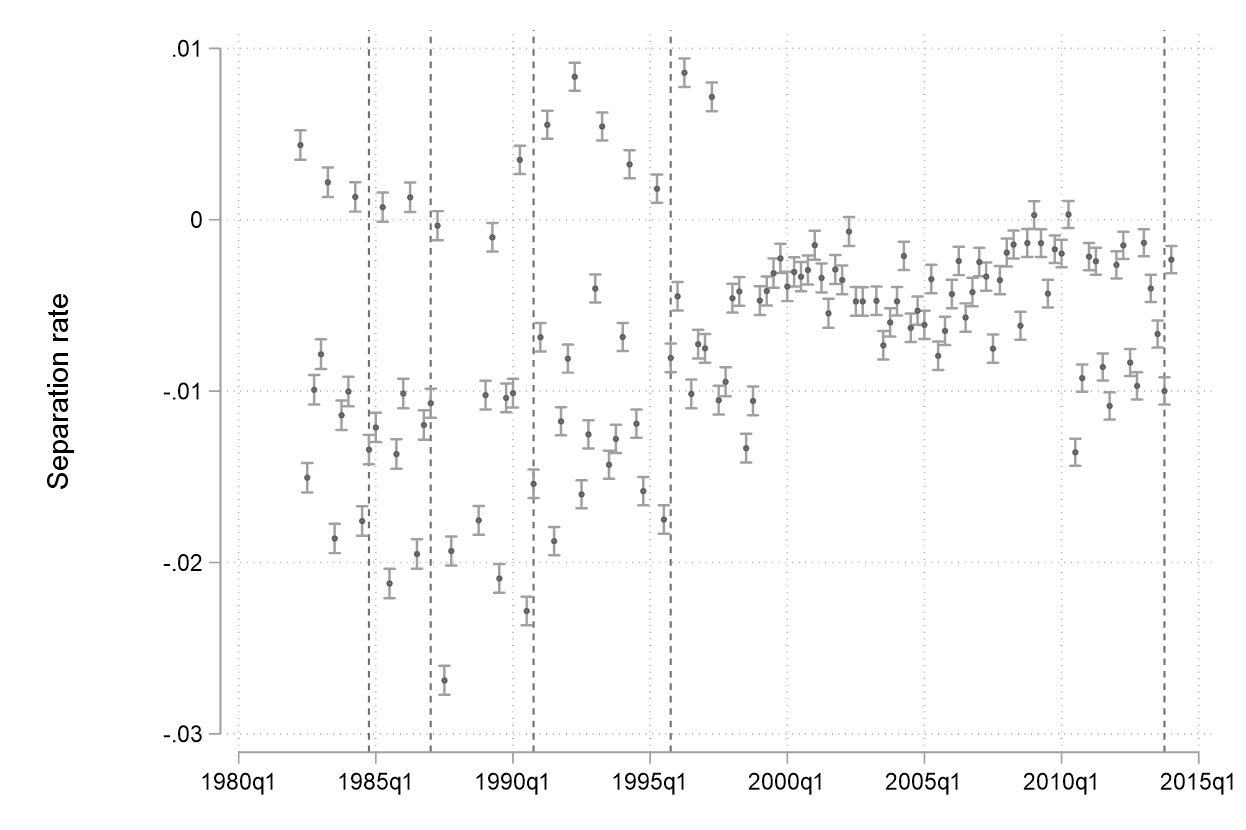
\includegraphics[width=0.8\textwidth]{../output/separation_rate_educ.png}
    \end{figure}

\end{frame}

\begin{frame}
    \frametitle{Difference in accession rates over time by education}

    \begin{figure}[]
        \centering
        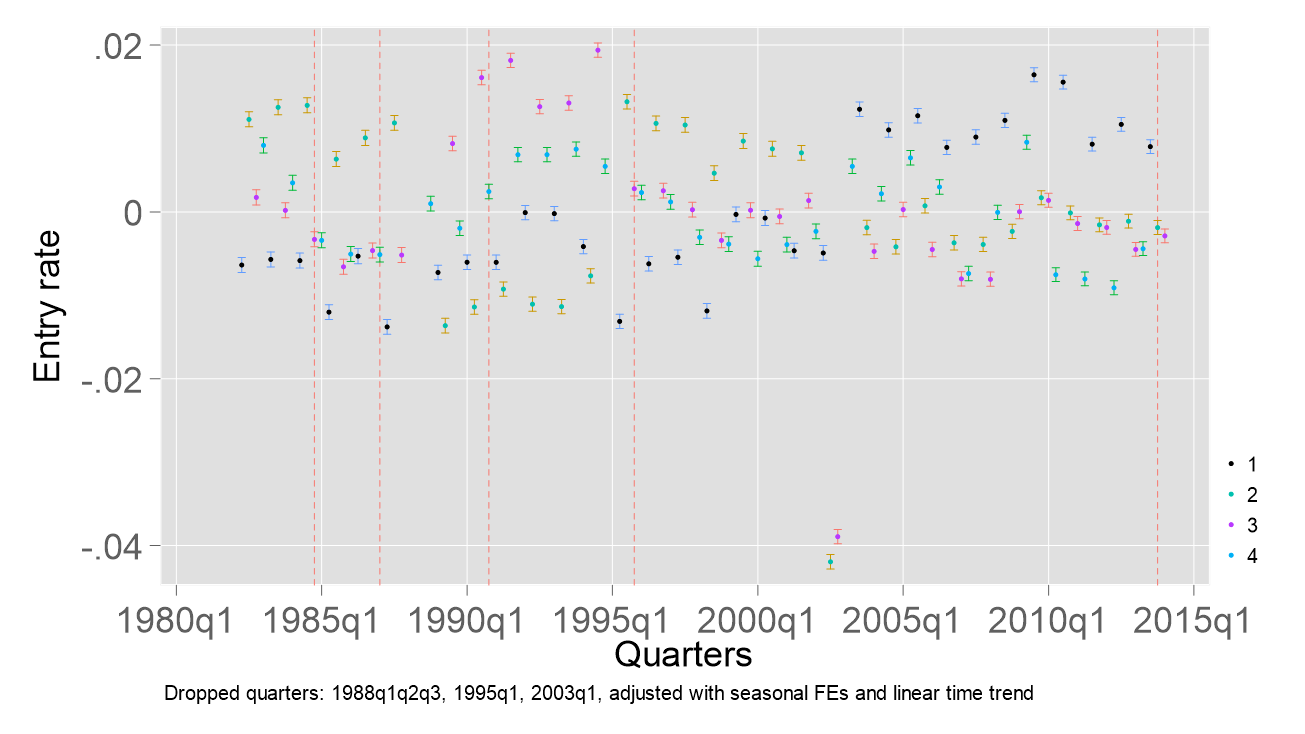
\includegraphics[width=0.8\textwidth]{../output/accession_rate_educ.png}
    \end{figure}

\end{frame}

\begin{frame}
    \frametitle{Difference in separation rates over time by median pay}

    \begin{figure}[]
        \centering
        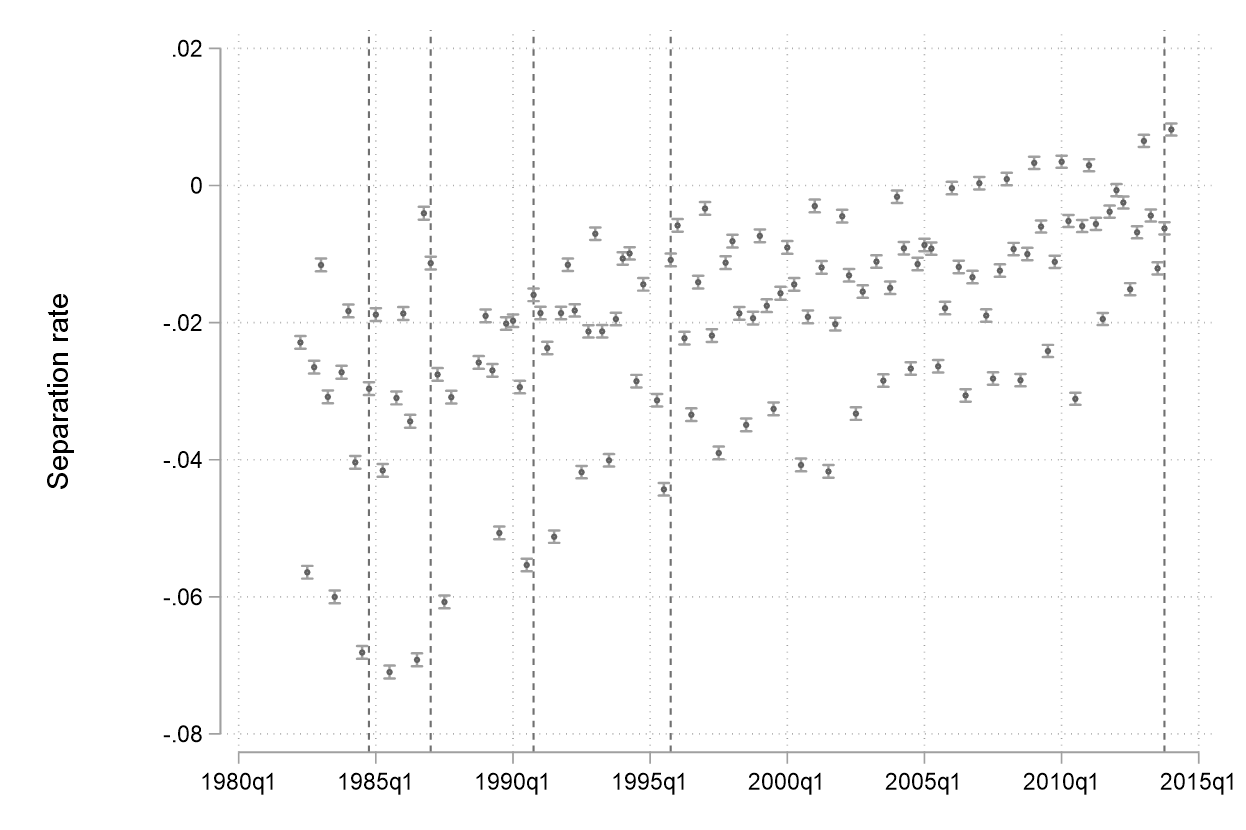
\includegraphics[width=0.8\textwidth]{../output/separation_rate_med_pay.png}
    \end{figure}

\end{frame}

\begin{frame}
    \frametitle{Difference in accession rates over time by median pay}

    \begin{figure}[]
        \centering
        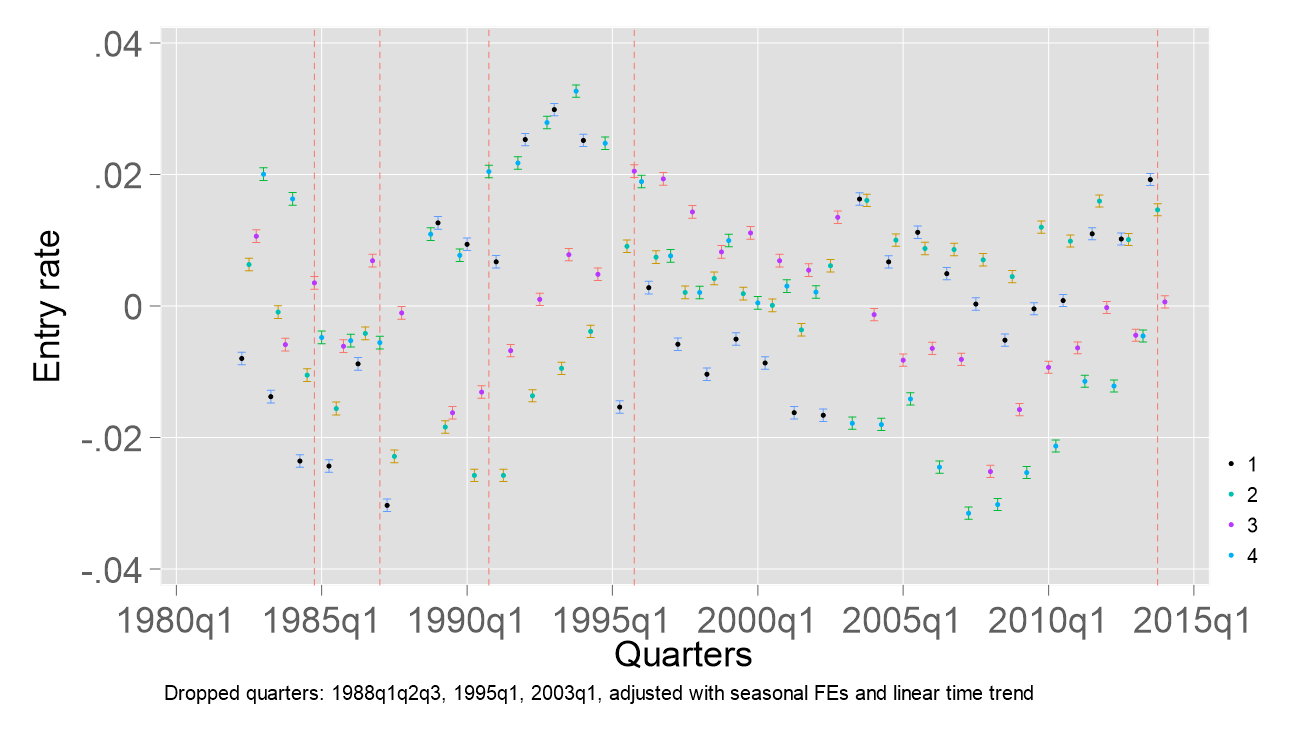
\includegraphics[width=0.8\textwidth]{../output/accession_rate_med_pay.png}
    \end{figure}

\end{frame}

\begin{frame}
    \frametitle{Difference in separation rates over time by tenure}

    \begin{figure}[]
        \centering
        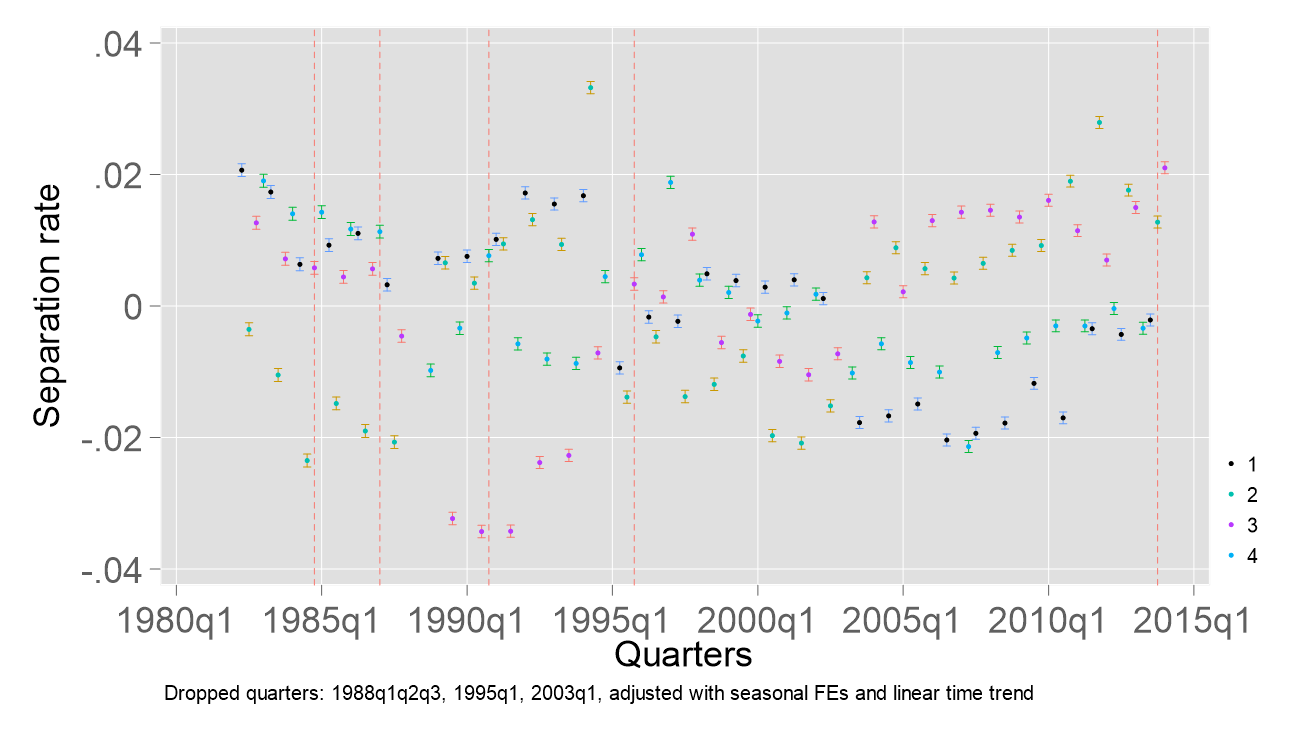
\includegraphics[width=0.8\textwidth]{../output/separation_rate_med_los.png}
    \end{figure}

\end{frame}

\begin{frame}
    \frametitle{Difference in accession rates over time by tenure (this doesn't make sense I think)}

    \begin{figure}[]
        \centering
        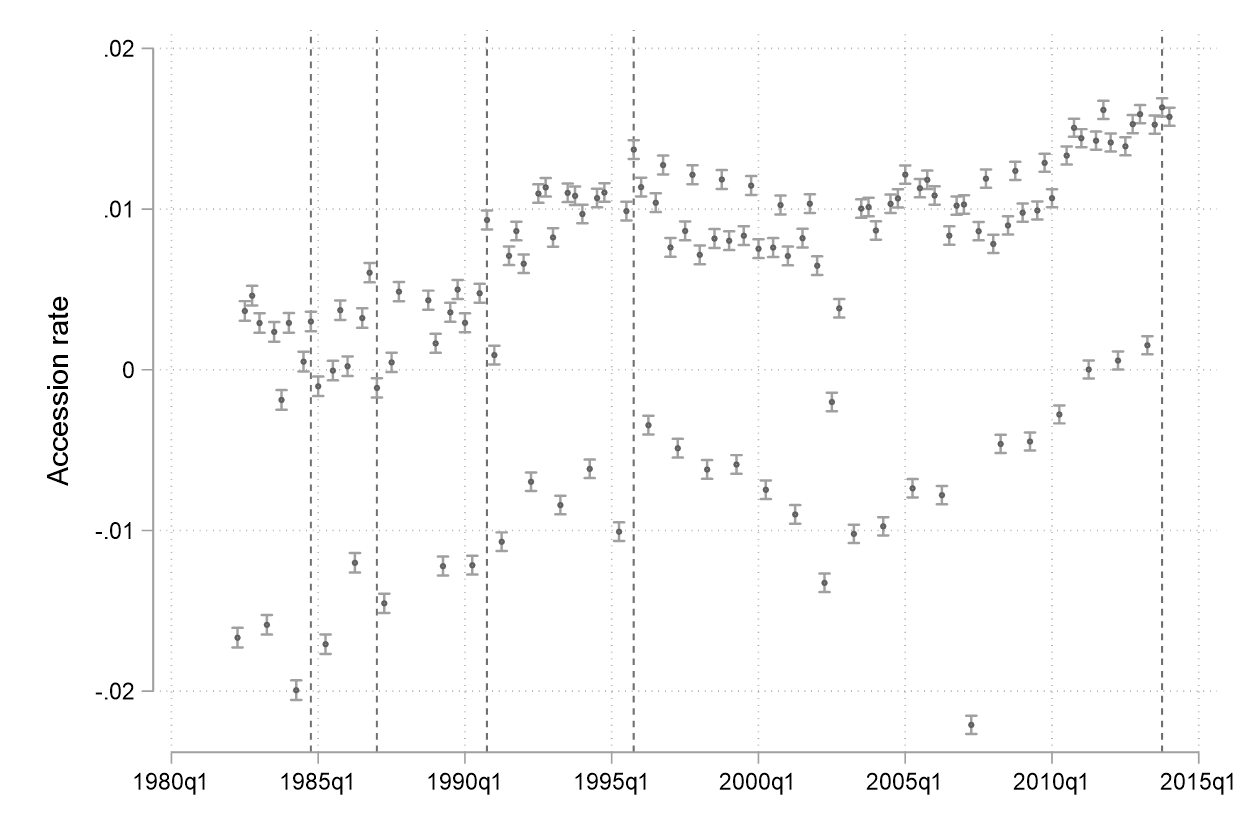
\includegraphics[width=0.8\textwidth]{../output/accession_rate_med_los.png}
    \end{figure}

\end{frame}


\end{document}
